\documentclass[12pt,fleqn,answers]{exam}
%\usepackage{pifont}
%\usepackage{dingbat,bbding}

\usepackage{amssymb}
\usepackage[intlimits]{amsmath}
\usepackage{epsfig}
\usepackage{upgreek}
\usepackage[super]{nth}
\usepackage[colorlinks=true,linkcolor=black,anchorcolor=black,citecolor=black,filecolor=black,menucolor=black,runcolor=black,urlcolor=black]{hyperref}
\usepackage[letterpaper, margin=0.75in]{geometry}
\addpoints
\boxedpoints
\pointsinmargin
\pointname{pts}
\usepackage{tikz}
\usepackage{tkz-euclide}
\usetikzlibrary{shapes.geometric}
\usetikzlibrary{calc}
\usepackage[final]{microtype}
\frenchspacing
\usepackage[american]{babel}
\usepackage[T1]{fontenc}
\usepackage[]{fourier}
\usepackage{isomath}
\usepackage{upgreek,amsmath}
\usepackage{amssymb}
\usepackage{graphicx}

\newcommand{\dotprod}{\, {\scriptzcriptztyle\stackrel{\bullet}{{}}}\,}

\newcommand{\reals}{\mathbf{R}}
\newcommand{\lub}{\mathrm{lub}} 
\newcommand{\glb}{\mathrm{glb}} 
\newcommand{\complex}{\mathbf{C}}
\newcommand{\dom}{\mbox{dom}}
\newcommand{\range}{\mbox{range}}
\newcommand{\cover}{{\mathcal C}}
\newcommand{\integers}{\mathbf{Z}}
\newcommand{\vi}{\, \mathbf{i}}
\newcommand{\vj}{\, \mathbf{j}}
\newcommand{\vk}{\, \mathbf{k}}
\newcommand{\bi}{\, \mathbf{i}}
\newcommand{\bj}{\, \mathbf{j}}
\newcommand{\bk}{\, \mathbf{k}}
\DeclareMathOperator{\Arg}{\mathrm{Arg}}
\DeclareMathOperator{\Ln}{\mathrm{Ln}}
\newcommand{\imag}{\, \mathrm{i}}

\usepackage{graphicx}
\usepackage{color}
%\shadedsolutions
%\definecolor{SolutionColor}{rgb}{1,0.72,0.46} %{0.8,0.9,1}
\newcommand\AM{\textsc{am}}
\newcommand\PM{\textsc{pm}}
     
\newcommand{\quiz}{4}
\newcommand{\term}{Fall}
\newcommand{\due}{Tuesday 5 September 13:20}
\newcommand{\class}{MATH 202, Fall \the\year}
\begin{document}
\large
\vspace{0.1in}
\noindent\makebox[3.0truein][l]{\textbf{\class}}
\textbf{Name:} \hrulefill \\
\noindent \makebox[3.0truein][l]{\textbf{In class work \quiz}}
\textbf{Row and Seat}:\hrulefill\\
\vspace{0.1in}


\noindent  In class work  \textbf{\quiz\/}  has questions \textbf{1} through  \textbf{\numquestions} \/ with a total of \textbf{\numpoints\/}  points.   
Turn in your work at the end of class  \emph{on paper}. This assignment is due \emph{\due}.

\vspace{0.1in}


\begin{questions} 

\question Define a region $Q$ of the xy plane by
$Q = \{(x,y) \mid 0 \leq y \leq 1-|x|,-1 \leq x \leq 1 \}$.

\begin{parts}

    \part [1] Sketch the region $Q$ in the xy plane.

    \begin{solution}[2.5in]
    \begin{center}
           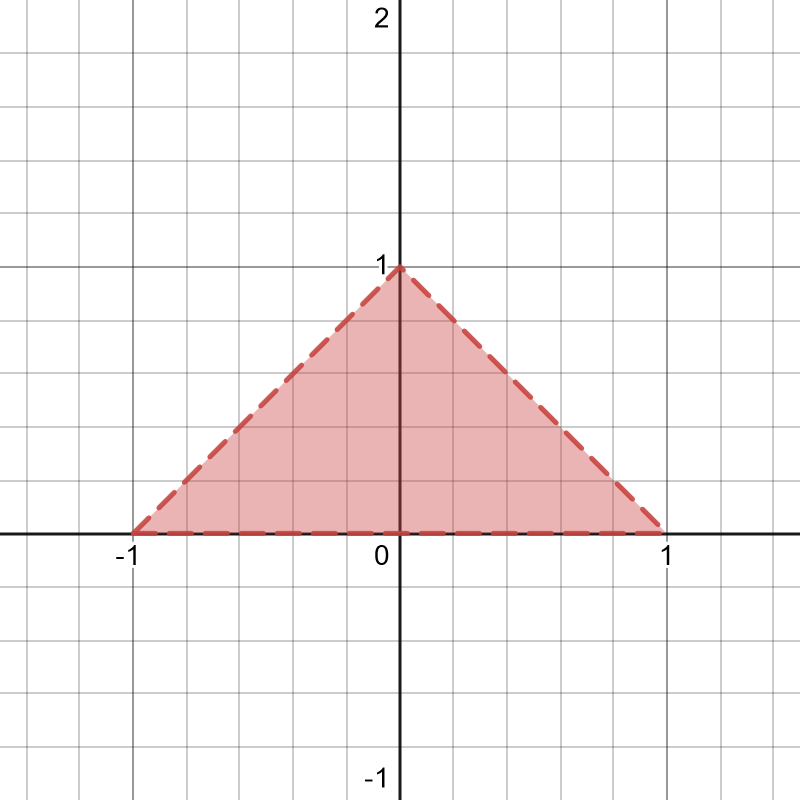
\includegraphics[scale=0.2]{desmos-graph(54).png}
  \end{center}
   \end{solution}

    \part [2] Make a conjecture about the location of the centroid of $Q$.
    Of course $\overline{x} \leq 107$ and $\overline{y} \leq 107$ is a conjecture, but 
    try for something more specific.
    \begin{solution}[2.5in]
    The region $q$ is symmetric with respect to the $y$ axis. Surely
    this means that $\overline{x} = 0$. 

    The triangle is bottom heavy, so the $y$ coordinate of the 
    center of should be less than $1/2$.
        
    \end{solution}

    \part [1] Use junior high math (no calculus) to find $\mbox{area}(Q)$.
    
    
    \begin{solution}%[2.5in]
    $        \mbox{area}(Q) = \frac{1}{2} \mbox{base} \times \mbox{height} = 1.$
    \end{solution}

    \newpage
    \part [1] Solve $M \overline{x} = \int_{-1}^1 x (1- |x|) \, \mathrm{d} x$,
    where $M$ is the area of $Q$, for $\overline{x}$. To evaluate the
    definite integral $\int_{-1}^1 x (1- |x|) \, \mathrm{d} x$, use a 
    fact about the integral of an odd function over a symmetric interval.
    \begin{solution}[2.5in]
        The integrand is odd and the interval is symmetric. So $\overline x = 0$.
        
        
        To show that the integrand is odd, we need to show that
        $y = x (1- |x|)$ and $- y = (-x) (1 - |-x|)$ are semantically the
        same.  We have
        \begin{align*}
        \left[ - y = (-x) (1 - |-x|) \right] 
           &\equiv  \left[- y = (-x) (1 - |x|) \right] && \mbox{(simplify absolute value)} \\
           &\equiv  \left[y = x (1 - |x|) \right] && \mbox{(multiply by -1)} 
        \end{align*}
    \end{solution}

    \part [1] Solve $M \overline{y} = \frac{1}{2} \int_{-1}^1 (1 - |x|)^2 \, \mathrm{d} x$,
    where $M$ is the area of $Q$, for $\overline{y}$. To  do this,
    use the fun fact that
    $\displaystyle
       \int |x| \, \mathrm{d}x = \frac{1}{2} x |x|.
    $
    \begin{solution}[2.5in]
    \begin{align*}
         M \overline{y} &= \frac{1}{2} \int_{-1}^1 (1 - |x|)^2 \, \mathrm{d} x,  && \mbox{(given)} \\
                              &=  \frac{1}{2} \int_{-1}^1 1  - 2 |x| + |x|^2 \, \mathrm{d} x,&& \mbox{(expand)} \\
                              &=  \frac{1}{2} \int_{-1}^1 1  - 2 |x| + x^2 \, \mathrm{d} x,  &&\mbox{(simplify $|x|^2$)}\\
                              &= \frac{1}{2}  \left(x - x |x| + \frac{1}{3} x^3 \right|_{x=-1}^{x= 1},  &&\mbox{(FTC)}\\
                              &= \frac{1}{2}  \left(1 - 1 + \frac{1}{3} \right) - \frac{1}{2}  \left(-1 + 1 - \frac{1}{3} \right) ,&&\mbox{(paste)} \\
                              &= \frac{1}{3}. &&\mbox{(arithmetic)}
                              \end{align*}
            Since $M=1$, we have $\overline y = \frac{1}{3}$.
    \end{solution}

\end{parts}
\end{questions}

\end{document}

